\chapter{基于车辆间作用力的网联自动驾驶车辆合流区分布式控制策略}
\label{chap:3}

本章建立在单车道场景下的车辆合流区分布式控制策略。首先对合流区域进行划分,将控制区划分为调整区和稳定区,然后针对两个区域的功能,分别提出了车辆在该区域的运动控制策略。此外,通过对合流区域的安全条件进行分析,给出了策略可以保证安全的初始状态条件范围。最后,通过仿真验证和敏感性分析,验证了本策略可以提升通行量、降低车均延误,并有较高的计算效率。

\section{问题描述}
\begin{figure}[htbp]
    \centering
    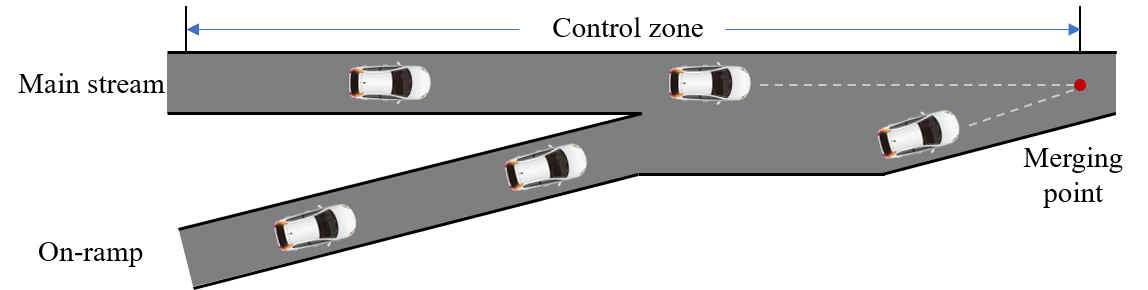
\includegraphics[width=\textwidth]{chap03/01.png}
    \caption{单车道合流场景}
    \label{fig:scenario}
\end{figure}
如图\ref{fig:scenario}所示的单车道合流区场景是合流区最基本的场景,常见于主线仅有一条车道可供汇入,或两条不同方向的匝道在汇入主线前进行合流的情况。网联环境下,通过车-车、车-路通信,车辆间可以共享信息,并接收控制指令,由路侧对车辆轨迹进行集中优化,以达到全局最优。然而,在实际场景中,所有车辆全部接受路端控制的场景是较难实现的。若仅共享信息,由车辆自主进行决策规划的分布式控制策略,则更为可行。同时,分布式的架构相对于集中式控制,在计算效率上具有显著优势,尤其是在较高的交通需求下。本章针对快速路场景下的单车道合流问题,面向纯网联自动驾驶车环境,提出了一种基于车辆间作用力的分布式控制策略。

模型的基本假设如下:
\begin{itemize}
    \item 控制区域内的车辆均为网联自动驾驶车辆,具有相同的车辆大小和动力学特性;
    \item 所有车辆可以通过车-车、车-路通信分享信息,并获取控制区内其它车辆的信息;
    \item 车辆在合流区域内的运动过程中,完全遵循本文所提出的控制策略。
\end{itemize}



\section{模型建立}
在本节中,我们将建立基于车辆间作用力的网联自动驾驶车辆合流区分布式控制模型。

\subsection{控制区划分}
\begin{figure}[htbp]
    \centering
    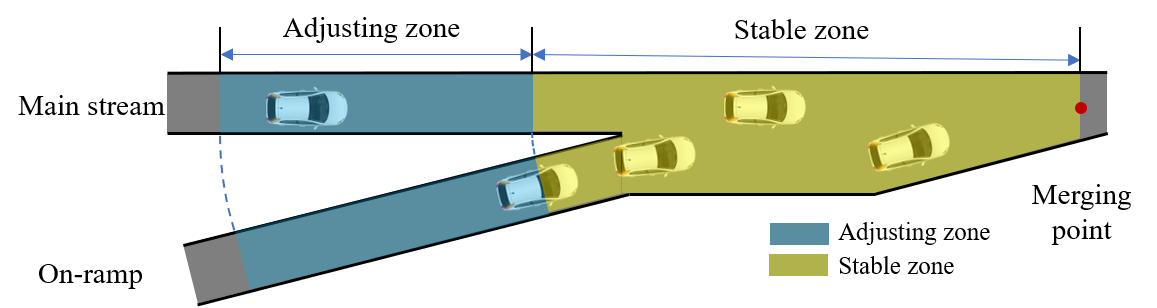
\includegraphics[width=\textwidth]{chap03/02.png}
    \caption{单车道合流场景}
    \label{fig:scenario_single_lane}
\end{figure}
如图\ref{fig:scenario_single_lane}所示,控制区被划分为两个区域,分别为调整区和稳定区。车辆在进入控制区后,依次通过两个区域,最终到达合流点。车辆在两个区域内受到的作用力是不同的。车辆根据自身和前车的位置与速度信息,计算受到的作用力,相应得到下一时刻的加速度。

\subsection{调整区控制策略}
在车辆通过合流区时,得到合流点的一个合理的通行顺序是十分重要的\cite{guler2014using}。调整区的设置,是为了调整车辆在合流点的通行顺序。

为了避免追尾碰撞,在通过合流点时,两辆车的车头时距应该大于一个最小的安全时间间隔。如果两辆车来自不同车道,相比于车辆在同一车道跟车的情况,该最小安全时间间隔应该更大。因此,该区域的基本控制思想是,让同一车道的临近车辆形成编队,以保持较小的车头时距通过合流点。通过减小车头时距,交通效率可以得到提升。

\subsubsection{车辆作用力设计}
调整区内的车辆的运动,由两类作用力决定。每辆车会受到一个基础作用力$F_0$的作用,该作用力基于车辆当前的速度$v$计算:
\begin{equation}
    F_0(v) = -mk_0(v-v_t)
    \label{eq:fund_force}
\end{equation}
其中,$v_t$是车辆的期望速度,$k_0$是正系数,控制基础作用力的大小,$m$是车辆的质量。力的正方向沿车辆的运动方向。车辆的期望速度大小是其前车的速度和自由流速度二者的较小值。基础作用力可以驱动车辆以期望速度运动。

此外,车辆需要与前车保持一个安全距离。因此,车辆之间的相互作用力$F_a$基于车辆与前车实时的车距$x$计算:
\begin{equation}
    F_{a}(x)=\left\{
    \begin{array}{cc}
        -m a_{\text {max }}^{-},                                                                           & x \leq x_{0}^{a} \\
        \min \left(m k_{a}\left(\frac{1}{x}-\frac{x_{e}^{2}}{x^{3}}\right), m a_{\text {max }}^{+}\right), & x>x_{0}^{a}
    \end{array}
    \right.
    \label{eq:inter_force_adjust}
\end{equation}
其中,$x$为车辆和前车的距离;$x_e$是稳定状态下(即$F_a(x_e)=0$)时对应的距离差;$a_{max}^-$和$a_{max}^+$分别是车辆最大减速度和加速度的绝对值;$k_a$是正系数,控制车辆间作用力的大小;$x_0^a$则是当$mk_a(\frac{1}{x}-\frac{x_e^2}{x^3})=-ma_{max}^-$时x的取值。车辆间作用力主要受车辆前车的影响。

距离差$x_e$与当前车辆的速度和车辆与前车的相对速度有关:
\begin{equation}
    x_{e}=t_1v+t_2(v-v_p)
    \label{eq:balance_dist}
\end{equation}
其中,$t_1$和$t_2$是系数,$v_p$是前车的速度。当车辆和前车在不同的车道时,考虑到安全条件,应该有更大的安全时间间隔。因此,在这种情况下$t_1$的取值应该更大。

\subsubsection{跟车关系}
\begin{figure}[htbp]
    \centering
    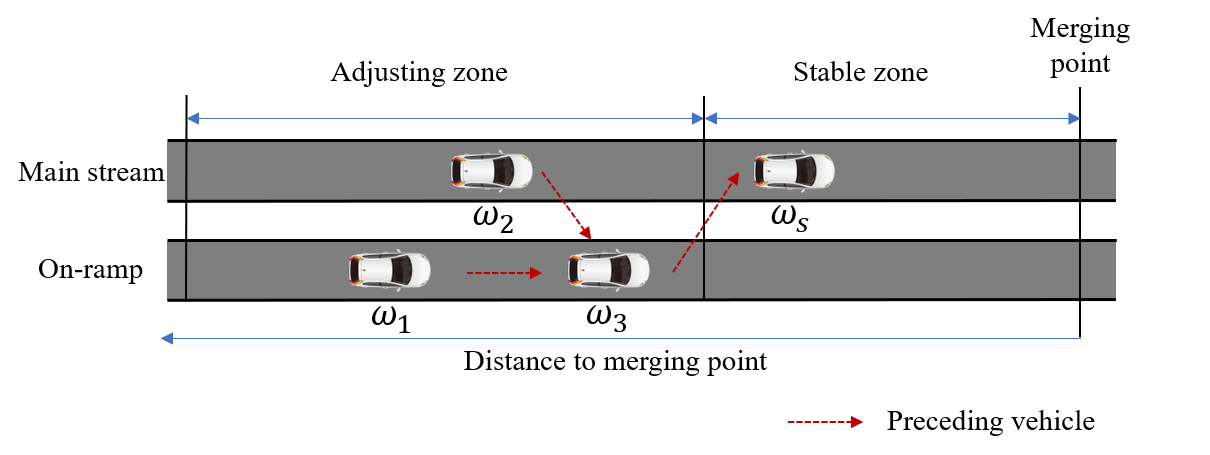
\includegraphics[width=\textwidth]{chap03/03.png}
    \caption{调整区内的跟车关系}
    \label{fig:follow_relation}
\end{figure}
不同于通常情况下对前车的定义,在调整区内,车辆之间的跟车关系是动态变化的。根据车辆所处位置,车辆之间的跟车关系可以分为以下三种情况,如图\ref{fig:follow_relation}所示:
\begin{itemize}
    \item 第一类:对于车辆$\omega_1$,调整区内,其所在车道上,有距离合流点更近的车辆。其中离$\omega_1$最近的车辆,即$\omega_3$,定义为$\omega_1$的前车。
    \item 第二类:对于车辆$\omega_2$,调整区内,其所在车道上,没有距离合流点更近的车辆。然而在另一条车道上,有距离合流点更近的车辆。其中离$\omega_2$最近的车辆,即$\omega_3$,定义为$\omega_2$的前车。
    \item 第三类:对于车辆$\omega_3$,调整区内,其所在车道上,没有距离合流点更近的车辆。在另一条车道上,也没有距离合流点更近的车辆。此时,$\omega_3$的前车定义为最后一辆离开调整区的车辆$\omega_s$。
\end{itemize}

\subsection{稳定区控制策略}
在车辆通过调整区后,车辆在合流点的通行顺序已经确定,即车辆进入稳定区的顺序。这一顺序不会在稳定区内被改变。稳定区的设置是为了让两条车道的车辆进行协同,以在到达合流点时顺利合流。

\subsubsection{虚拟车道}
\begin{figure}[htbp]
    \centering
    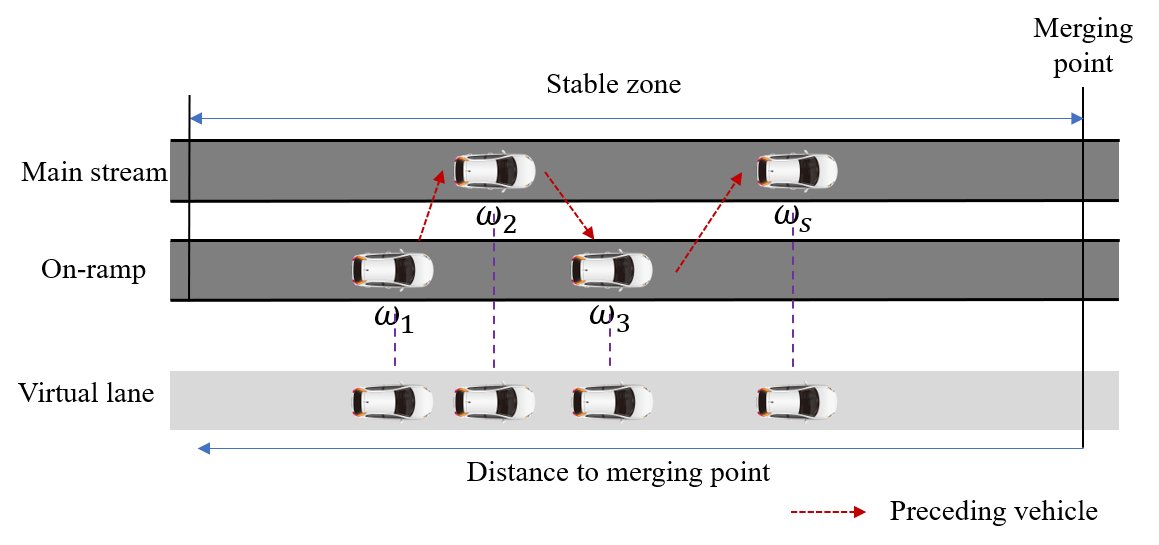
\includegraphics[width=\textwidth]{chap03/04.png}
    \caption{虚拟车道映射}
    \label{fig:virtual_lane}
\end{figure}
稳定区引入了虚拟车道的概念,以便更好地确定车辆的前车,保证车辆在合流点的安全。在稳定区内的所有车辆,根据其在稳定区内的位置,被映射至虚拟车道。借助车-车和车-路通信,车辆可以共享他们的位置,得到其在虚拟车道上的顺序,从而确定其前车。在稳定区内,车辆的前车定义为其在虚拟车道上的前车。如图\ref{fig:virtual_lane}所示,车辆$\omega_3$、$\omega_2$、$\omega_1$的前车分别为$\omega_s$、$\omega_3$、$\omega_2$。



\subsubsection{车辆作用力设计}
与调整区类似,在稳定区内,车辆的运动同样到基础作用力$F_0$和车辆间作用力$F_s$的影响。稳定区内基础作用力的计算与调整区内相同,即\ref{eq:fund_force}。而车辆间作用力$F_s$的计算则有所不同:
\begin{equation}
    F_{s}(x)=\left\{
    \begin{array}{cc}
        -m a_{\text {max }}^{-},                                                                      & x \leq x_{0}^{s} \\
        \min \left(m k_{s}\left(\ln{x}-\frac{x_{e}\ln{x_e}}{x}\right), m a_{\text {max }}^{+}\right), & x>x_{0}^{s}
    \end{array}
    \right.
    \label{eq:inter_force_stable}
\end{equation}
其中,$x$是在虚拟车道中车辆和前车的距离;$x_e$是稳定状态下(即$F_s(x_e)=0$)时对应的距离差,计算方式如\ref{eq:balance_dist};$k_s$是正系数,控制车辆间作用力的大小;$x_0^s$则是当$mk_s(\ln{x}-\frac{x_e\ln{x_e}}{x})=-ma_{max}^-$时x的取值。在稳定区中,车辆间作用力也主要受车辆前车的影响。

\subsection{安全条件分析}
在实际交通环境中,车辆突然并入或者紧急刹车的情况是不可避免的。在这种情况下,需要保证车辆的安全。因此,有必要分析车辆在本控制策略下的安全条件。在本节中,我们将通过理论推导,给出车辆在控制区内保证安全的初始状态条件范围。

假设车辆$\omega_j$和其前车$\omega_i$在同一车道行驶,且车速相同。在紧急状况下,前车$\omega_i$开始以最大减速度减速直到停车。当车距缩小到$x_e$时,车辆间作用力会变为负值,在其作用下$\omega_j$会开始减速。当车距进一步缩小到$x_0$(在稳定区内为$x_0^s$,在调整区内为$x_0^a$)时,车辆的减速度大小会达到最大值$a_{max}^-$,如\ref{eq:inter_force_adjust}和\ref{eq:inter_force_stable}所示。将$\omega_j$减速过程中,车距由$x_e$缩小到$x_0$的时间记为$t_{r}$。

为了便于分析,假设一个较实际情况更为保守的情况,即在$t_{r}$时间内,$\omega_j$并没有减速。若在这种情况下满足无碰撞,则在实际应用\ref{eq:inter_force_adjust}和\ref{eq:inter_force_stable}的情况下也会满足无碰撞。

将车辆$\omega_j$的速度记为$v_j$,前车$\omega_i$的速度记为$v_i$。当车距缩小到$x_e$时,$\omega_i$的减速距离为
\begin{equation}
    x_{i}=\frac{v_{i}^{2}}{2 a_{\max }^{-}}
    \label{eq:decel_dist_i}
\end{equation}
$\omega_j$在时间$t_r$内以恒定速度$v_j$行驶,之后以最大减速度减速,其行驶距离为
\begin{equation}
    x_{j}=v_{j} t_{r}+\frac{v_{j}^{2}}{2 a_{\max }^{-}}
    \label{eq:decel_dist_j}
\end{equation}
如果可以满足$x_j\leq x_i + x_e$,则$\omega_j$和$\omega_i$之间不会发生碰撞。

在时间间隔$t_r$内,$\omega_j$的行驶距离和$\omega_i$的行驶距离之差,应该等于二者距离的变化:
\begin{equation}
    v_j t_r - v_i t_r + \frac{a_{max}^-t_r^2}{2} = x_e - x_0
    \label{eq:dist_diff}
\end{equation}

将$v_j-v_i$记作$\Delta v$,将\ref{eq:decel_dist_i}, \ref{eq:decel_dist_j}和\ref{eq:dist_diff}代入$x_j\leq x_i + x_e$,可以得到安全条件的一般表达式:
\begin{equation}
    \frac{1}{2 a_{\max }^{-}}\left(\frac{2 a_{\max }^{-} x_{e}+(\Delta v)^{2}}{2 v_{j}}\right)^{2}-\frac{1}{2 a}(\Delta v)^{2}-x_{e}+x_{0}>0
    \label{eq:safe_condition}
\end{equation}

如果初始状态下,车队处于稳定状态,即$\Delta v=0$,则\ref{eq:safe_condition}可以简化为:
\begin{equation}
    \frac{1}{2 a_{\max }^{-}}\left(\frac{2 a_{\max }^{-} x_{e}}{2 v_{j}}\right)^{2}-x_{e}+x_{0}>0
    \label{eq:safe_condition_stable}
\end{equation}
当$\Delta v=0$时,$x_e=t_1 v_j$,此时\ref{eq:safe_condition_stable}变为:
\begin{equation}
    \frac{a_{\max }^{-} t_{1}^{2}}{2}-x_{e}+x_{0}>0
    \label{eq:safe_condition_stable_xe}
\end{equation}
化简可得
\begin{equation}
    v_j < \frac{x_0}{t_1} + \frac{at_1}{2}
    \label{eq:safety_final}
\end{equation}
如果等式\ref{eq:safety_final}成立,则车辆可以保证安全。

\section{案例分析}

\subsection{仿真设计}
本节通过仿真实验,验证本章所提出的控制策略的效果。
本策略与先来先服务策略\cite{au2010motion}进行对比。先来先服务策略根据车辆进入控制区的顺序确定车辆的通行顺序。
为了评价两种策略的性能,在仿真时选取车均延误和总通行量作为评价指标。车辆的延误定义为车辆在控制区内的通行时间与其在自由流状态下的通行时间之差。总通行量定义为仿真时段内离开控制区的总车辆数。

为了全面评价策略在不同交通需求下的性能,仿真中分别选取了从低到高的不同交通需求、主线和匝道流量是否平衡等不同场景。为了简化计算,车辆的质量被设置为单位质量。调整区和稳定区的长度都设置为200米。车辆的最大速度为25$m/s$。车辆的最大加速度和减速度大小均为5$m/s^2$。每次仿真时长为30分钟。在仿真时段内,车辆的到达时间服从泊松分布。

\subsection{仿真结果}
\begin{table}[]
    \begin{tabular}{cccccccc}
    \hline
    \multicolumn{2}{c}{交通需求(veh/h)} & \multicolumn{3}{c}{通行量(veh/h)} & \multicolumn{3}{c}{车均延误(veh/h)} \\ \hline
    主线              & 匝道              & 对照策略    & 本策略     & 提升比例(\%)    & 对照策略      & 本策略     & 降低比例(\%)   \\ \hline
    900             & 900             & 1626    & 1632    & 0.37        & 11.66     & 10.78   & 7.55       \\
    1008            & 1008            & 1716    & 1848    & 7.69        & 47.45     & 28.76   & 39.39      \\
    1080            & 1080            & 1752    & 1854    & 5.82        & 46.42     & 34.99   & 24.62      \\
    1188            & 1188            & 1740    & 1908    & 9.66        & 59.04     & 36.8    & 37.67      \\
    1260            & 1260            & 1716    & 1956    & 13.99       & 96.76     & 66.1    & 31.69      \\ \hline
    1440            & 900             & 1740    & 1950    & 12.07       & 81.72     & 56.9    & 30.37      \\
    1440            & 1080            & 1710    & 1926    & 12.63       & 100.58    & 81.38   & 19.09      \\
    \hline
    \end{tabular}
    \caption{车辆通行量和车均延误}
    \label{tab:sim_res}
    \end{table}

\ref{tab:sim_res}展示了对照策略(先来先服务)和本策略下,不同交通需求下的通行量和车均延误。
当需求较低时,本策略相较于对照策略,在通行量和车均延误指标上的优势不大。但是,在高交通需求的情况下,本策略显著提升了通行量,降低了车均延误。例如,在主线和匝道的交通需求均为1260veh/h时,本策略相较于对照策略,通行量提升了13.99\%,车均延误降低了31.69\%。合流点的通行能力得到较大提升。在主线和匝道流量不平衡的需求下,本策略相较于对照策略,也在相应指标上取得了显著提升。当主线流量为1440veh/h,匝道流量为900veh/h时,本策略相较于对照策略,通行量提升了12.07\%,车均延误降低了30.37\%。这体现出本策略在不同交通需求下的通用性和可靠性。
此外,本策略在计算效率上也与对照策略接近,二者均可在0.1s内完成计算。
\subsection{敏感性分析}
在调整区内,车辆的通行顺序被动态调整并确定。这一区域的长度对于策略的效果有着重要影响。本节对调整区的长度进行敏感性分析,以评估其对策略效果的影响。主线和匝道的流量均被设置为1260veh/h。
\begin{figure}[htbp]
    \centering
    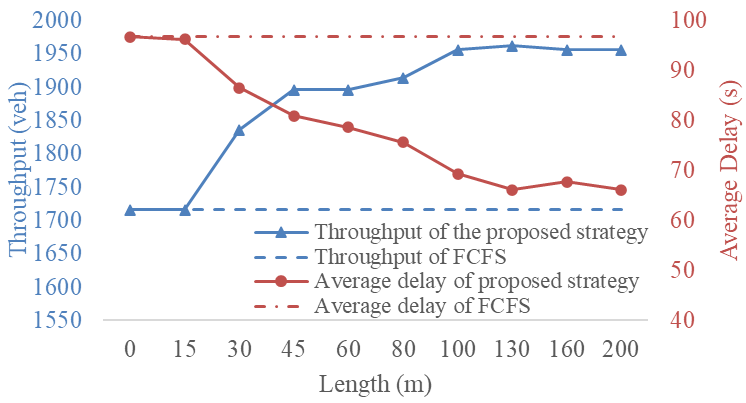
\includegraphics[width=\textwidth]{chap03/05.png}
    \caption{调整区长度的敏感性分析}
    \label{fig:sensitivity}
\end{figure}
仿真结果如图\ref{fig:sensitivity}所示。当调整区长度较短时,车辆没有充足的空间进行通行顺序的调整。因此,本策略的效果与对照策略较为接近。随着长度的增加,本策略在通行量和车均延误指标上的优势逐渐显现。但当调整区长度达到130m后,长度继续增加时,本策略的效果提升较小。这是因为调整区内的空间已足够使车辆形成一个较为合理的通行顺序。这说明130m的调整区长度已足够保证本策略有令人满意的效果。

\section{本章小结}
本章提出了一种基于车辆间作用力的分布式控制策略,使网联自动驾驶车辆可以在单车道合流区内实现协同高效合流,实现了系统最优和计算效率间的平衡。控制区被划分为调整区和稳定区。车辆通过合流点的顺序在调整区内被确定。在稳定区内,车辆根据该顺序被映射至虚拟车道。车辆根据区域内的规则确定前车,并通过网联环境下收集到的前车的信息(位置和速度),决定自车的加速度。这一过程被构建为“车辆间作用力”模型。数值仿真表明,相较于“先来先服务”策略,本策略显著提升了通行量,降低了车均延误,并且具有较高的计算效率。
